\documentclass{chi-ext}
% Please be sure that you have the dependencies (i.e., additional LaTeX packages) to compile this example.
% See http://personales.upv.es/luileito/chiext/

%% EXAMPLE BEGIN -- HOW TO OVERRIDE THE DEFAULT COPYRIGHT STRIP -- (July 22, 2013 - Paul Baumann)
% \copyrightinfo{Permission to make digital or hard copies of all or part of this work for personal or classroom use is granted without fee provided that copies are not made or distributed for profit or commercial advantage and that copies bear this notice and the full citation on the first page. Copyrights for components of this work owned by others than ACM must be honored. Abstracting with credit is permitted. To copy otherwise, or republish, to post on servers or to redistribute to lists, requires prior specific permission and/or a fee. Request permissions from permissions@acm.org. \\
% {\emph{CHI'14}}, April 26--May 1, 2014, Toronto, Canada. \\
% Copyright \copyright~2014 ACM ISBN/14/04...\$15.00. \\
% DOI string from ACM form confirmation}
%% EXAMPLE END -- HOW TO OVERRIDE THE DEFAULT COPYRIGHT STRIP -- (July 22, 2013 - Paul Baumann)

\title{Portrait Pigeon: An Interactive Photo Messaging Wall for Seniors}

\numberofauthors{3}
% Notice how author names are alternately typesetted to appear ordered in 2-column format;
% i.e., the first 4 autors on the first column and the other 4 auhors on the second column.
% Actually, it's up to you to strictly adhere to this author notation.
\author{
  \alignauthor{
  	\textbf{Robin Brewer}\\
  	\affaddr{Northwestern University}\\
  	\affaddr{2240 Campus Drive}\\
  	\affaddr{Evanston, IL 60208 USA}\\
  	\email{rnbrewer@u.northwestern.edu}
  }
  \vfil
  \alignauthor{
  	\textbf{Moritz Gellner}\\
  	\affaddr{Northwestern University}\\
  	\affaddr{2240 Campus Drive}\\
  	\affaddr{Evanston, IL 60208 USA}\\
  	\email{moritzgellner2014@u.northwestern.edu}
  }
  \vfil
  \alignauthor{
  	\textbf{Anne Marie Piper}\\
  	\affaddr{Northwestern University}\\
  	\affaddr{2240 Campus Drive}\\
  	\affaddr{Evanston, IL 60208 USA}\\
  	\email{ampiper@northwestern.edu}
  }
}

% Paper metadata (use plain text, for PDF inclusion and later re-using, if desired)
\def\plaintitle{Portrait Pigeon An Interactive Photo Messaging Wall for Seniors}
\def\plainauthor{Robin Brewer}
\def\plainkeywords{Older adults, gestures, interactive wall, lightweight communication}
\def\plaingeneralterms{Design, Human Factors}

\hypersetup{
  % Your metadata go here
  pdftitle={\plaintitle},
  pdfauthor={\plainauthor},  
  pdfkeywords={\plainkeywords},
  pdfsubject={\plaingeneralterms},
  % Quick access to color overriding:
  %citecolor=black,
  %linkcolor=black,
  %menucolor=black,
  %urlcolor=black,
}

\usepackage{graphicx}   % for EPS use the graphics package instead
\usepackage{balance}    % useful for balancing the last columns
\usepackage{bibspacing} % save vertical space in references


\begin{document}

\maketitle

\begin{abstract}
Considerable research has studied online communication for older adults. As we age, it gets more difficult to communicate due to minor and sever vision, cognitive and mobility impairments. At the same time there's more opportunities to create more lightweight IX online for older adults. A valuable approach to do so is to embed this IX in familiar or culturally-relevant artifacts and practices. We have designed Portrait Pigeon which supports lightweight communication by interacting w/physical photos on a wall. We describe this general approach

??include general terms?

Exploration of lightweight communication for older adults

Older adults with vision impairments have difficulty navigating complex graphical interfaces for communication such as e-mail platforms and social networking sites. Further, older adults with mobility impairments experience difficulty physically getting to a computer just to access such digital communication platforms. While efforts have been made to simplify the aesthetics of the interfaces, these solutions are not exploring challenges such as mobility and accessibility of the overall experience. We have designed Portrait Pigeon, a system that embeds communication into familiar environments of older adults focusing on their preference for displaying photos. We describe how a highly-customizable interactive photo wall was designed using depth-sensing technology.
\end{abstract}

\keywords{\plainkeywords}

\category{H.5.m}{Information interfaces and presentation (e.g., HCI)}{Miscellaneous}. 

\terms{\plaingeneralterms}


% =============================================================================
\section{Introduction}
% =============================================================================
Embedding online IXin in online artifacts is a rich area for ubicomp design which allows OA to IXt with tech in their daily routines + environments. 

[[reframe this sentence + replace. the point is that they don't need to learn something new]] Technology is often designed for mainstream users meaning other populations such as older adults have to adapt and learn something new, or be excluded. Ubiquitous computing becomes a rich design area which allows older adults to interact with technology by embedding computers in their daily environment and routines. OA value keeping in touch and storing non-digital photographs \cite{}. Drawing on these values we describe the design of an interactive photo wall for seniors that allows them to send lightweight text and voice messages. 

Our research extends upon work using pictures and everyday objects for communication through interactive displays. A case study of older adults has demonstrated that they value storing and displaying photos \cite{Swan2008}. One key observation was the semi-permanent display of photos on walls, meaning pictures are not moved often once a display space is found for them. We leverage the permanency of photo locations with Portrait Pigeon, but also provide a simple interface for linking static photos w/dynamic online IXn.

A number of examples look like re-purposing static walls, tables, and objects for IXn through depth sensing (e.g. Microsoft Kinect).

Not only can one object such as a picture frame be manipulated for interaction, but researchers have explored the re-purposing of any object for input using immediate calibration \cite{Corsten2013}. While this is convenient, users must train the program with repeated trials. Existing examples of interactive environments and surfaces using gesture interaction include LightBeam \cite{Lightbeam2012}, [[delete LightSpace, add depth-camera as a touch sensor paper]] LightSpace \cite{Wilson2010}, and Magic Finger \cite{Yang2012}. 

Prior work has looked at making surfaces such as walls + tables IXive. A more interesting approach is to make the actual objects IXive.

We extend re-purposing of objects by focusing on the use of photo frames for email messaging through text and voice. Also, we simplify the training of the interactive environment through a simple interface where seniors map locations of their natural environment to the e-mail address of the person in the picture frame. This paper continues by describing how 1) the system was implemented and how it can be customized to address individual needs of users, 2) modes of lightweight messaging, and 3) feedback mechanisms.

The contribs of this work are tailoring IX for OAs with various disabilities, linking diff modes of lightweight messages, and prototyping feedback mechanisms. 

[[blur faces]]

% =============================================================================
\section{Portrait Pigeon}
% =============================================================================
We developed a prototype of Portrait Pigeon as shown in Figure 1. Below we describe the features of the system and how they can be easily customized for individual users depending on their level of ability and comfort.

\begin{figure}
	\centering
	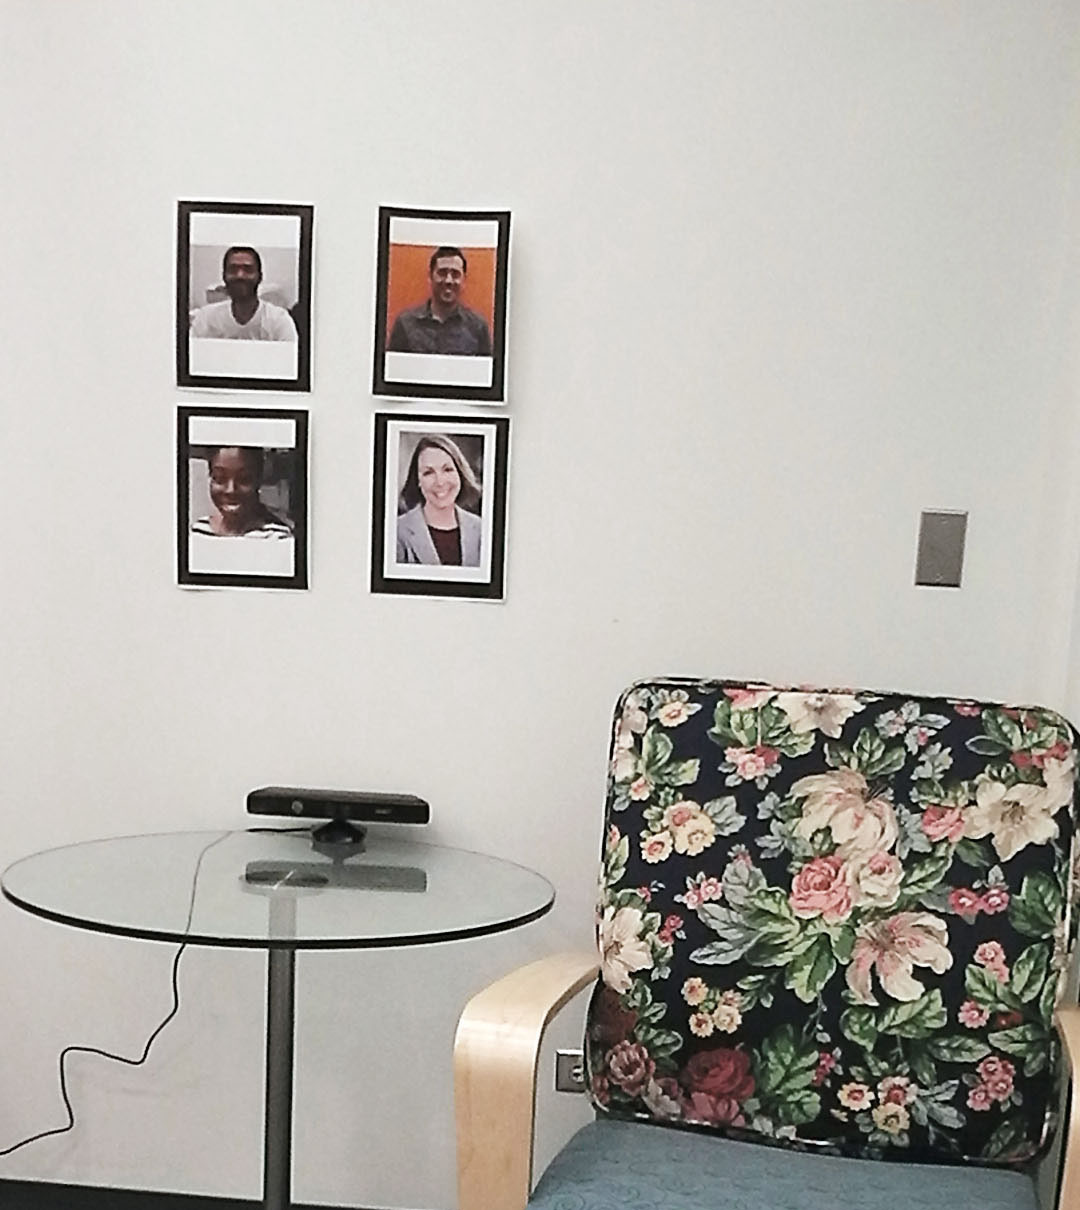
\includegraphics[width=0.3\textwidth]{photo-chair.JPG}
	\caption{Portrait Pigeon setup with the Kinect facing the user}
\end{figure}

\subsection{Gesture Recognition}
The prototype uses a Microsoft Kinect, the SimpleOpenNI library, and Processing to basic IXn w/physical photos. The camera detects gestures targeted towards photos by calculating arm movement relative to the user's torso. For example, if a picture on a quadrant coordinate system is in the top left quadrant, a gesture is recognized when a hand (right or left) is placed above the left elbow. The relative positioning and recognition of gestures can be customized for individual older adults. For example, lower quadrant recognition can be changed from \textit{below the hip} to \textit{below the waist}. This customization is particularly important for older adults with limited range of motion because they may not be able to fully extend towards photos positioned at extreme ends of the wall. 

The Kinect is positioned on the same wall as the photos, facing the user (Fig. 1). This positioning was favored over the Kinect facing the wall to allow gesture recognition of a photo directly in front of the user, without the need of multiple depth-sensors. We extend this by re-purposing photo frames for email... [insert GUI screenshot -- current/initial on top and a dynamic one on the bottom, link to @_rnbrewer mailto: ___]

\subsection{Set-up}
An important design challenge is creating a setup that is simple for OAs + their fams to initialize. In order to know where the photos are located, Portrait Pigeon  must first obtain a picture of the environment. Prior to sending the first message, users must upload a picture of their photo wall and tag people in the photos \textbf{[[INSERT FIGURE OF OLD(top) NEW(bottom) GUI]]}. If there is more than one person in the photo, it is up to the user to define which person they would want to send a message to. Also if a picture is moved, the system allows for easy re-uploading of the wall setup. This can also be extended to pictures in frames and not on walls as long as the frames are on the same side of the wall as the Kinect. While we recognize this may be a limitation for older adults without a digital camera or cell phone, additional depth-sensors would allow us to replace this manual setup with an automatic setup, where a second Kinect would capture the location and content of pictures on the photo wall. Furthermore, computer vision could be used to implement automatic facial recognition so that Portrait Pigeon could automatically associate the framed pictures with stored contact information. This would reduce its reliance on such a rigid coordinate system in which pictures can be placed; instead, contacts could be mapped to arbitrary and more precise spatial areas.

[[depth image side-by-side]]

\subsection{Sending a Message}
% -----------------------------------------------------------------------------
Through Portrait Pigeon, seniors can send email messages to family and friends. These messages can either be in text or voice format. Currently we explore lightweight pre-created text email messages that are sent when a user gestures towards that person's picture on their wall. Such messages let the person in the portrait know that their loved one is thinking of them. For more customized input, the system could use Kinect's built-in microphone to record a voice message. The voice message could be emailed directly or use speech-to-text technology to send a text email message. Here we focus on email because it is the communication platform that most seniors are currently using \cite{Pew2012}. However the existing reliance on text and computer access could pose challenges to people with low vision or mobility impairments. Not only does Portrait Pigeon help seniors with physical impairments and low vision, but also cognitive impairments because they wouldn't need to remember the complex processes of accessing email. We posit that Portrait Pigeon is easy to learn because it draws on the social practice of acknowledging someone with gesture (e.g. a wave hello) to initiate communication with them online (e.g. sending an email message).

Flexible enough to support calls to FB, etc. 


% =============================================================================
\section{Feedback}
% =============================================================================
Audio is played to inform the user that an email message has been sent. For older adults who may have hearing impairments, audio feedback could be supplemented with visual feedback from a small short-range projector facing the photo display \cite{Wilson2010}. Using the Kinect's depth sensor, we could approximate the position on the wall that a user is currently pointing at and project a mark onto that spot, so that the user knows which area s/he is currently pointing to (Fig. 2). This would make the system more interactive and intuitive to use, which is important to engage older adults that are less inclined to experiment with new technology.

\begin{figure}
    \centering
    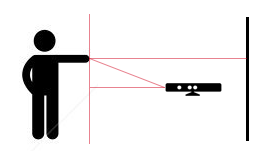
\includegraphics[width=0.3\textwidth]{kinect_diag.png}
    \caption{Inferring hand position using depth sensing}
\end{figure}

\section{Pilot Testing with Older Adults}
Pilot testing was conducted with seniors of an assisted living community. To test the initial concept, we used photos of community staff and introduced Portrait Pigeon as a way to send 'thinking-of-you' messages of appreciation to the staff members. We saw that seniors were hesitant to use Portrait Pigeon fearing it may take too much time or that they didn't have a message to send to the staff in the photos. From the two users willing to try the system we observed that the positioning of the user with respect to the Kinect was an issue, with a sharp decline in hand tracking accuracy if the depth camera was not positioned directly between the photo wall and the user. Lastly, we found that one user expected to be able to record and send an audio message after receiving the audio feedback which was intended to indicate that the text email message was sent. Based on feedback from this initial testing, we are incorporating visual feedback to halo a person's hand to guide them on how to reach the target. Based on the existing coordinates of a user's shoulder and skeleton, we use geometric calculations to recognize the angle of a person's hand and where it is pointing. We are also taking advantage of the embedded microphone in the Kinect that could record voice messages of users and email those to the target person in the photo. 

[[add more complex geometry to the figure + how the calculations would be managed]]

% =============================================================================
\section{Conclusion and Future Work}
% =============================================================================
This paper presents Portrait Pigeon, a ubiquitous lightweight messaging platform for seniors that leverages existing in-home photo displays [[put this in the abstract  reframe throughout the paper]]. PP lowers the barrier of online IX for OAs 
Portrait Pigeon will lower the barrier of entry for older adults who aren't familiar w/going online or have difficulty using the comp. The interactive photo wall supports lightweight comm with family and friends. We believe it has the potential to let OA see the value of online comm platforms (e.g. Facebook, Twitter, and e-mail) and interact w/... because it is embedded into the environment of seniors.  We highlight the ease of customization (body recognition, setup, platform dependency, and feedback) in Portrait Pigeon which is especially important due to the wide range in abilities of older adults. In the future we will expand the system to incorporate reciprocal communication where the people tagged in the portraits can send messages to seniors, explore different communication platforms, and supplement audio feedback with visual feedback.	

\balance
\bibliographystyle{acm-sigchi}
\bibliography{sample}

\end{document}